\section{Impostazioni generali}

Tutte le istruzioni fornite sono riferite all'utilizzo dell'applicativo con il tema chiaro e con il sistema impostato in lingua italiana. Se si ha la necessità di cambiarlo si veda la sezione 2 e 3 delle impostazioni generali sottostanti.

Il sistema in alto a destra presenta due simboli: una rotella e un omino stilizzato. La prima è la rotella che dà accesso alle impostazioni di cui sotto e l'omino stilizzato permette l'accesso come tecnico al sistema (sezione Tecnico 6.1).

Una volta cliccata la rotella, si apre un menù a tre voci con le caratteristiche modificabili dall'utente del sistema:
\begin{enumerate}
    \item La scala di grandezza del testo
    \item La modalità di visualizzazione del sistema chiara o scura
    \item La lingua del sistema
\end{enumerate}

\begin{figure}[H]
  \centering
  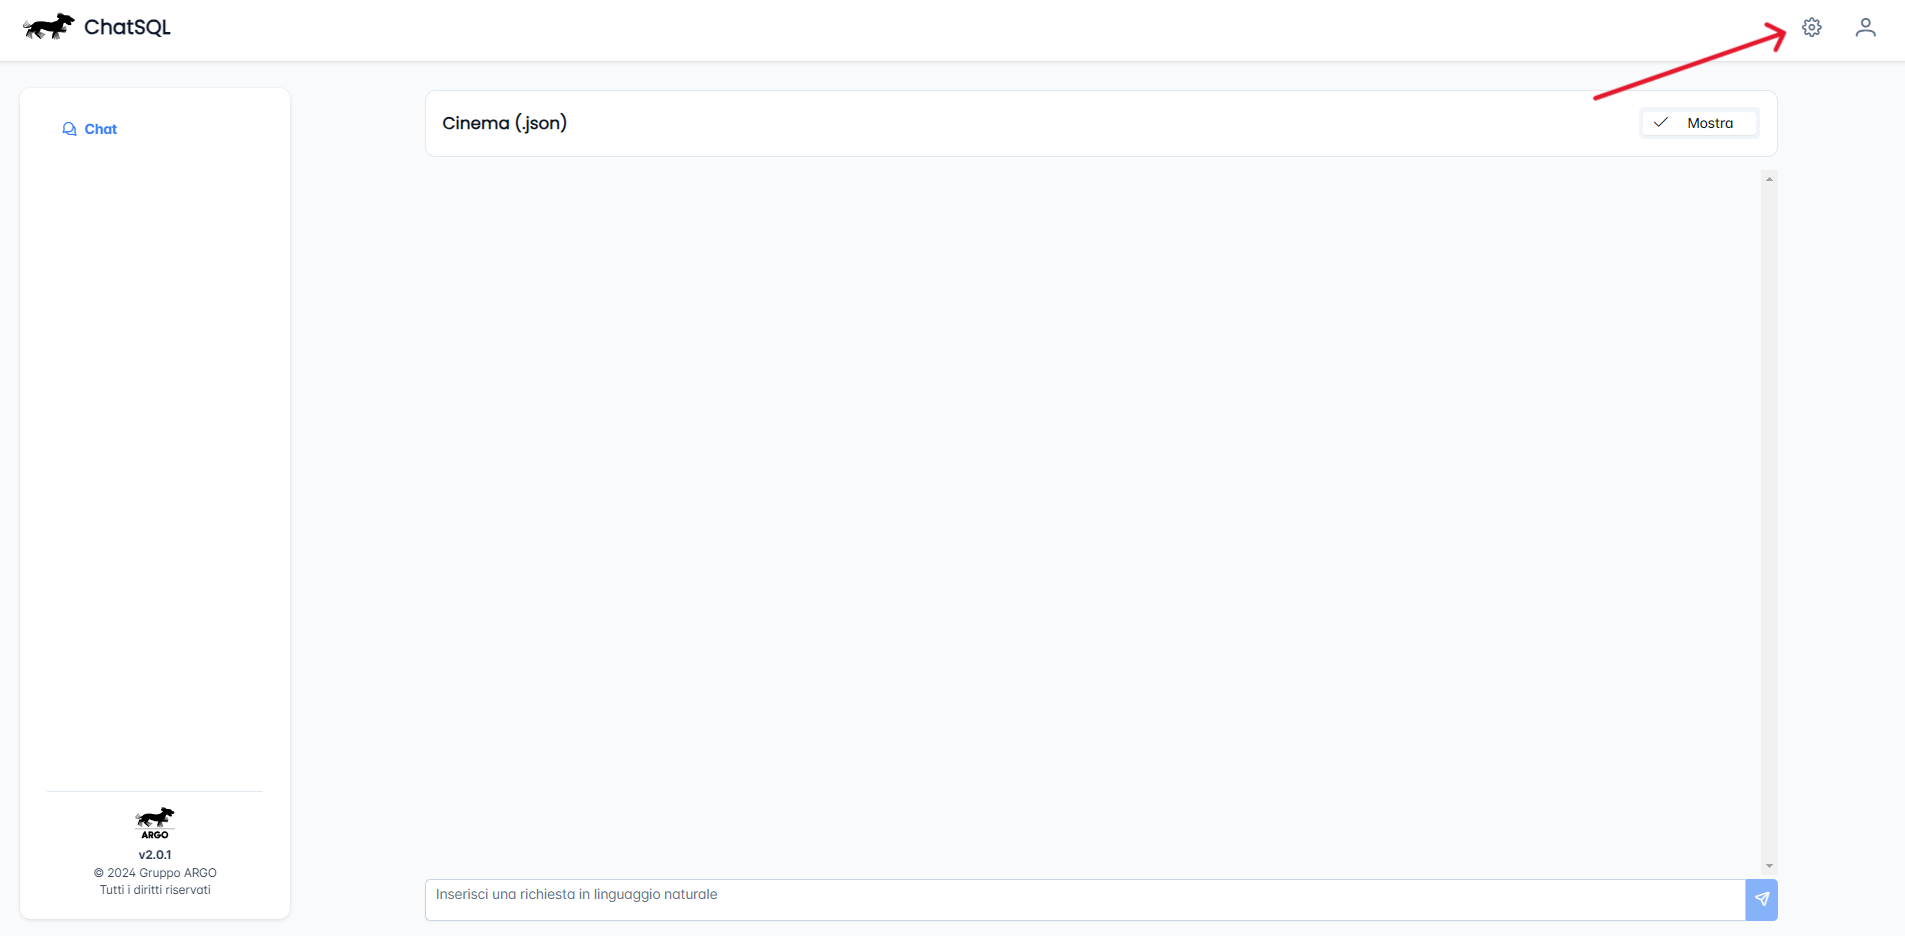
\includegraphics[width=1\textwidth]{assets/chat_generale.png}
  \caption{Icona impostazioni}
\end{figure}

\subsection{Scala di grandezza del testo}

Il sistema permette di far scegliere all'utente la grandezza dei caratteri del testo tramite una scala di 5 misure diverse. Per modificare la grandezza è necessario cliccare il ``-'' o il ``+'' presenti affianco alla voce ``Scala'' che permettono rispettivamente di rimpicciolire o ingrandire il testo.

\begin{figure}[H]
    \centering
    %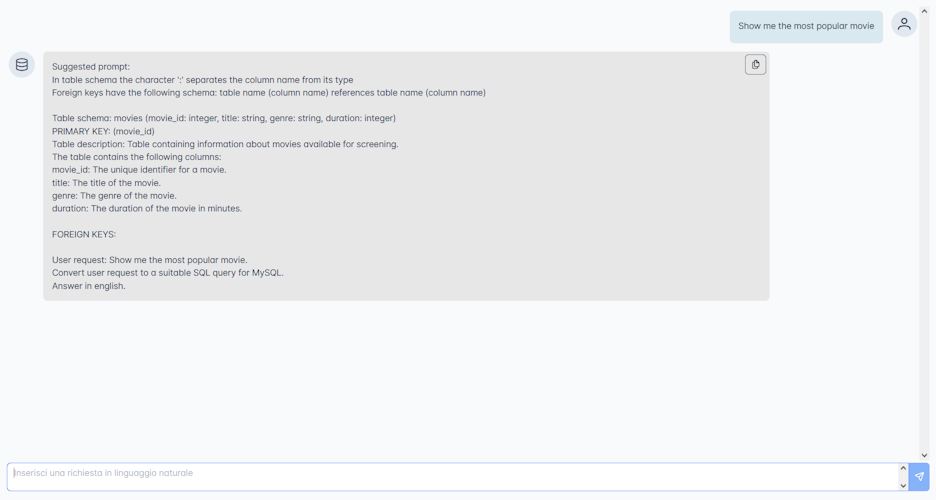
\includegraphics[width=1\textwidth]{assets/chat_example.png}
    \caption{Immagine con freccia nella scala}
  \end{figure}

\subsection{Modalità di visualizzazione del sistema chiara o scura}

Il sistema permette di impostare la modalità chiaro/scuro. Di default la modalità è chiara, ovvero il colore di sfondo del sistema è il bianco, ma è possibile cliccare nel pulsante affianco alla voce ``Modalità scuro'' per attivare il tema scuro a sfondo nero.

\begin{figure}[H]
    \centering
    %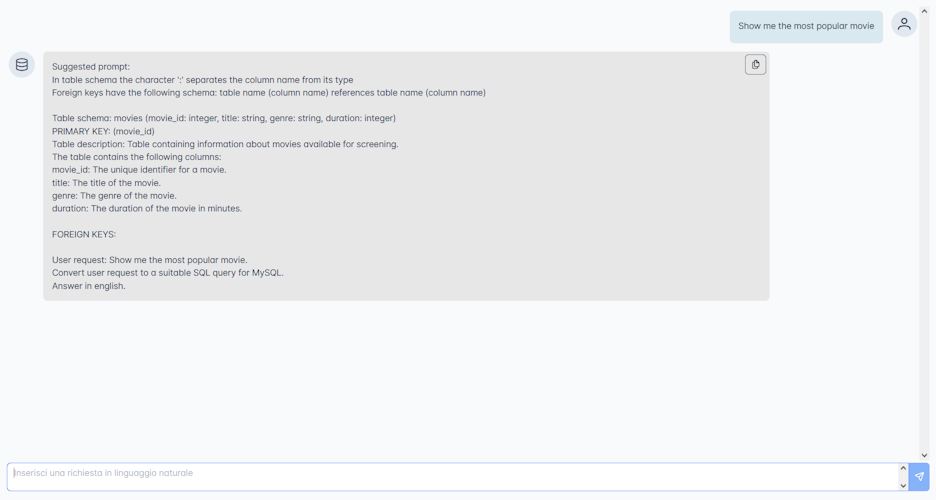
\includegraphics[width=1\textwidth]{assets/chat_example.png}
    \caption{Immagine con freccia nel modalità notte}
  \end{figure}

\subsection{Lingua del sistema}

Il sistema permette di impostare la lingua con cui il sistema si presenta, per esempio le parole dei bottoni o le voci dei menù. Questa voce non influenza la lingua con cui viene restituito il prompt dal sistema (si veda per questo la sezione 6.2.4). Le lingue possibili sono l'italiano e l'inglese di cui l'inglese è quella di default.

\begin{figure}[H]
    \centering
    %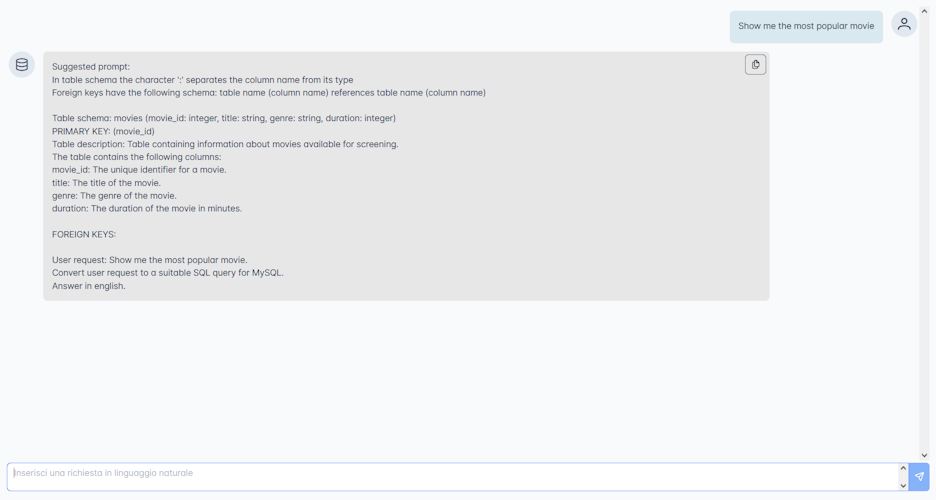
\includegraphics[width=1\textwidth]{assets/chat_example.png}
    \caption{Immagine con freccia nella lingua}
  \end{figure}

Per uscire dalle impostazioni è necessario cliccare la ``x'' in alto a destra e si tornerà al sistema con le impostazioni scelte.
